

\ifdefined\maindoc
% Do nothing (we are inside main.tex)
\else
\documentclass[12pt]{report}
\usepackage[a4paper,margin=1in]{geometry}
\usepackage[utf8]{inputenc}
\usepackage[T1]{fontenc}
\usepackage{amsmath,amssymb,amsthm}
\usepackage{booktabs}
\usepackage{setspace}
\usepackage{graphicx}
\usepackage{subcaption}
\usepackage{enumitem}
\usepackage{placeins}
\usepackage{hyperref}
\usepackage{array}
\usepackage{makecell}
\usepackage{algorithm}
\usepackage{algpseudocode}
\usepackage[backend=biber,style=ieee,citestyle=numeric-comp,sorting=none]{biblatex}
\addbibresource{references.bib}
\newtheorem{theorem}{Theorem}
\newtheorem{lemma}[theorem]{Lemma}
\newtheorem{definition}[theorem]{Definition}
\newtheorem{proposition}[theorem]{Proposition}
\newtheorem{remark}[theorem]{Remark}
\onehalfspacing
\graphicspath{{figures/}}
% Standalone-only fallbacks so Chapter~\ref{...} renders as the right number outside the
% main thesis. Under \maindoc these are skipped and the real labels in main.tex resolve.
\makeatletter
\newlabel{ch:input-module}{{3}{1}{}{Doc-Start}{}}
\newlabel{ch:probability-toolkit}{{5}{1}{}{Doc-Start}{}}
\makeatother
\begin{document}
\title{Sub-graph Decomposition: Diamond Processing Module}
\fi

\newcommand{\infl}{\mathrm{infl}}
\newcommand{\Anc}{\mathrm{Anc}}
\newcommand{\topi}{\mathrm{topi}}
\newcommand{\hkey}{\mathrm{hkey}}
\newcommand{\ED}{\mathcal{E}_D}



\section{Introduction}
\label{sec:dd-intro}

The Input Module returns a validated graph object that carries the network topology together with its layered iteration sets and ancestry closures. All analysis modules in the framework consume this object directly as is. 

The Network Decomposition Module, when invoked, extends the graph object with the network's decomposition structure. 
Like input processing, this is a network pre-processing step whose objective is to identify all instances of a specified subgraph pattern in the input DAG network. 

\subsection{Decomposition in Complex Networks}
\label{sec:dd-family}

Real infrastructure networks are rarely trees. Their components connect to
and depend on many others at once, and the interactions between them
overlap rather than branch cleanly \cite{ouyang2014interdependent,buldyrev2010cascade}. Redundancy strategies are the obvious
case: a robust network deliberately supplies more than one route to the
same goal, so paths diverge and reconverge by design. Process networks and
hierarchical flows behave the same way, with a component feeding several
downstream dependencies while itself depending on shared upstream outputs.
As the system grows, overlapping paths accumulate and the connectivity web
thickens.

Graph-based analysis methods almost always do some form of decomposition,
and for large networks with complicated connectivity it is a practical
necessity \cite{perez2018sixty}. Broadly, decomposition breaks a network into substructures that
are easier to handle than the whole, and methods differ in what they do
with those substructures. Some strategies aim to reduce: a substructure is replaced by a
single equivalent element, so the network shrinks while the analysis stays
exact. Other decomposition methods work by partition: the network is divided into units of work sized
for the solver, and the pieces are processed in turn. Beyond either,
decomposition can give a more compact representation of the network,
storing a repeated substructure once rather than every time it appears,
without losing the overall structure. Depending on how the decomposed units are
defined, they can also support localised investigation, such as confining
a sensitivity study to one part of the system without needing to run
analysis against the full network.

There is no universal correct unit of decomposition; a decomposition
method defines its own target substructure and partitions the network in
those terms. In the classic series--parallel reduction, the reliability
formula replaces each series or parallel pair with a single equivalent
component and the network shrinks pair by pair
\cite{satyanarayana1985linear}. The units here are the series and parallel
pairs themselves. When the network is not series--parallel, that reducible
structure is missing, and the factoring approach manufactures it:
conditioning on a single component splits the problem into the
component-working and component-failed cases, and the method recurses on
each until it becomes reducible
\cite{moore1956reliable,satyanarayana1983factoring,page1988practical}.
Polygon-to-chain reductions extend the same idea, widening what can be
collapsed in one step beyond the plain series and parallel pairs
\cite{wood1985polygon}.

In dynamic programming the unit is the tree: a tree decomposition arranges
the network into small overlapping bags of nodes connected in a tree, each
interacting with the rest of the graph only through its neighbours, which
is exactly the subproblem structure a dynamic program can process in a
single sweep \cite{robertson1986graphminors}. Working over bags rather
than the whole graph is what makes exact reliability computation feasible
on networks as large as metropolitan transit systems
\cite{goharshady2020treewidth}.

The framework's default decomposition unit is the \emph{diamond}: a
fork--join subgraph where paths in the network fan out from a common node and fan back in at a node further downstream. IPA's decomposition is partition-forward, that is, each identified diamond is returned as a localised graph object of the same form as the full network, and can be handed to any analysis module in the framework on its own. Secondarily, a diamond can serve as a reductive unit, since a solved diamond can stand in for its subgraph as a single equivalent component.


\section{Preliminaries and Definitions}
\label{sec:dd-prelim}

Identification works directly on the unified graph object of Chapter~\ref{ch:input-module}. From it the module reads the DAG $G=(V,E)$ and the iteration sets $L = \{L_1,\dots,L_k\}$, whose validity is the Convergence Guarantee proved there. It also reads the ancestry closures, where the ancestor closure $\Anc(v)$ is self-inclusive by construction so that $v \in \Anc(v)$ for every node, and the fork and join classifications, a fork having fan-out above one and a join fan-in above one. The node value map travels with the object, but identification reads it in one place only, the exclusion rule of Section~\ref{sec:dd-isdet}. The edge value map plays no part at all and is accepted only so the module's signature matches the rest of the framework.

\begin{definition}[Topological index]
\label{def:topi}
Given the iteration sets $L$, define $\topi : V \to \{1,\dots,|V|\}$ by numbering nodes in increasing order across layers and in sorted node order within each layer. Every node receives a distinct integer, so $\topi$ is a strict total order on $V$ refining the layered order.
\end{definition}

\begin{definition}[Conditioning context]
\label{def:context}
A conditioning context $E \subseteq V$ is a set of nodes treated as fixed while assessing the relatedness of their descendants. Identification starts from $E=\varnothing$ and extends the context one node at a time as it recurses.
\end{definition}

\begin{definition}[Unconditioned influence set]
\label{def:infl}
For a node $p$ and context $E$,
\[
\infl(p,E) \;=\; \Anc(p)\setminus E .
\]
Two parents $p, q$ of a join are \emph{structurally correlated under $E$} when $\infl(p,E) \cap \infl(q,E) \neq \varnothing$, that is, when some node upstream of both is not held fixed by the context. When the intersection is empty no unfixed node can reach both parents, and the two incoming paths are structurally unrelated.
\end{definition}

\begin{definition}[Diamond]
\label{def:diamond}
A diamond is a triple $D = (R, C, \ED)$. The relevant node set $R \subseteq V$ spans the reconvergent pattern. The conditioning set $C \subseteq V$ records which nodes identification fixed, or found already fixed, to isolate the pattern. The edge list $\ED \subseteq E$ is induced on $R$ by the membership rule constructed in Section~\ref{sec:dd-edges} and characterised in Lemma~\ref{lem:isolation}.
\end{definition}

The module returns diamonds at two levels. A \texttt{DiamondsAtNode} record attaches to one join node its diamond together with the join's \emph{non-diamond parents}, meaning the parents found unrelated to every reconvergent group at that join. The map \texttt{root\_diamonds} collects these records for every join of $G$ at the top level, and the diamonds recorded there are the network's \emph{maximal diamonds}, identified at the network's own joins rather than inside another diamond. Separately, every diamond identified at any level, top-level or nested, is stored exactly once in \texttt{unique\_diamonds}, keyed by the structural identity of Section~\ref{sec:dd-identity}. Each entry carries the diamond's fully analysed local structure (Section~\ref{sec:dd-representation}), and nested reconvergence appears as entries referencing other entries, so the store is a hierarchy rather than a flat list.

\section{A Configurable Target Subgraph}
\label{sec:dd-genericity}

The algorithms of this module are written against a definition of the special subgraph, not against the diamond in particular. \label{sec:dd-extension}Three predicates carry that definition. \texttt{is\_det} decides when a node's reachability counts as already settled, \texttt{shared\_fork} decides what counts as a correlating structure worth conditioning on, and \texttt{components} with $\infl$ decides when two parents count as independent. The identification and build algorithms do the same work whatever these predicates say. They find every subgraph of the input network whose structure satisfies the supplied properties, so a user can redefine the target around the network characteristics they care about and the module as it stands will decompose the network in those terms.

Apart from the \texttt{is\_det} test, identification never reads the value map, and the structures it emits only carry the map restricted to their spans. The decomposition therefore behaves identically under all three of the framework's value types (deterministic, interval, and p-box), which is required of every module sitting between input processing and the analysis toolkits.

The diamond is the framework's default target, and as shipped the predicates encode the definitions of Section~\ref{sec:dd-prelim}.

\section{The Identification Algorithm}
\label{sec:dd-algorithm}

The identification procedure \texttt{new\_identify} is the first of the module's two algorithms. It visits every join node of $G$ once at the top level and recursively inside diamonds, and Algorithm~\ref{alg:new-identify} shows its recursive skeleton.

\begin{algorithm}[htbp]
\caption{Recursive diamond identification (skeleton)}
\label{alg:new-identify}
\begin{algorithmic}[1]
\Require join node $v$, context $E$, admissible parent set $P$
\Ensure list of \texttt{DiamondsAtNode} for $v$ under $E$
\State partition $P$ into groups by pairwise $\infl(\cdot,E)$ intersection \Comment{union--find; Section~\ref{sec:dd-partition}}
\ForAll{groups $G$ with $|G| \geq 2$}
    \State $f \gets$ covering candidate of $G$ with minimum $\topi$ \Comment{Section~\ref{sec:dd-fork}}
    \State construct diamond $D$ for $(v, G, f)$ under boundary $B = E \cup \{f\}$ \Comment{Section~\ref{sec:dd-edges}}
    \State look up $D$ in \texttt{unique\_diamonds} by its identity key; reuse if present \Comment{Section~\ref{sec:dd-identity}}
    \ForAll{join nodes $j$ interior to $D$}
        \State recurse on $(j, B, \text{parents of } j \text{ within } D)$ \Comment{residual reconvergence}
    \EndFor
\EndFor
\State singleton groups become non-diamond parents of $v$
\end{algorithmic}
\end{algorithm}

\subsection{Conditioning only where correlation exists}
\label{sec:dd-targeted}

By Definition~\ref{def:infl}, two parents of a join are correlated under $E$ exactly when their unconditioned influence sets intersect. Extending the context with a node removes that node from every influence set, which is the factoring move of Section~\ref{sec:dd-family} applied inside a single network. The algorithm conditions only where an intersection actually exists and only on one node at a time. Nothing is enumerated exhaustively, and recursion stops as soon as the parents in view are pairwise unrelated.

\subsection{Independence partitioning}
\label{sec:dd-partition}

At join $v$ with admissible parents $P$ and context $E$, the procedure \texttt{components}$(P,E)$ evaluates $\infl(p,E) \cap \infl(q,E)$ for every pair and merges classes by union--find whenever the intersection is non-empty. The groups it returns are the connected components of the correlation relation (Theorem~\ref{thm:grouping}), and distinct groups share no unconditioned ancestry at all (Theorem~\ref{thm:disjoint}), so each group can be decomposed on its own. Parents in singleton groups are related to nothing at $v$ and become the join's non-diamond parents.

\subsection{Fork selection}
\label{sec:dd-fork}

For a correlated group $G$, \texttt{shared\_fork}$(G,E)$ tallies every node that \emph{covers} at least two members of the group. Coverage arises in two ways. A fork node may lie in the ancestry of two or more members, which is the symmetric picture of a diamond. A member of $G$ may instead be an ancestor of another member, the asymmetric case where the reconverging paths share no third node and the covering node is one of the parents itself. Both are genuine reconvergence and both are tested. Candidates already in $E$ are skipped, since fixing an already fixed node does nothing, and so are candidates excluded by \texttt{is\_det} (Section~\ref{sec:dd-isdet}).

Among the surviving candidates the algorithm selects the one with minimum topological index, the covering node closest to the sources. Conditioning as far upstream as possible leaves the largest part of the group's shared structure intact downstream of the chosen node, where it stays available for reuse. Because $\topi$ is a strict total order the minimum is unique.

\subsection{The recursive loop}
\label{sec:dd-loop}

Selecting fork $f$ for group $G$ at join $v$ produces the diamond, constructed under the extended boundary $B = E \cup \{f\}$. It does not end the work at $v$, because conditioning on $f$ need not resolve all correlation inside the pattern. Any interior join whose parents remain correlated under $B$ gives rise to a nested diamond, found by the same procedure with the extended context. The recursion bottoms out when every group everywhere is a singleton, and Theorem~\ref{thm:termination} bounds its depth by $|V|$.

\subsection{Edge construction and isolation}
\label{sec:dd-edges}

The diamond for group $G$ at join $v$ under boundary $B$ spans
\[
R \;=\; \{v\} \cup G \cup \bigcup_{p \in G}\Anc(p),
\]
the join, the group, and everything upstream of the group, with induced edge list
\[
\ED \;=\; \bigl\{\, (u,w) \in E \;:\; u,w \in R,\;\; w \notin B,\;\; (w \neq v \;\text{or}\; u \in G) \,\bigr\}.
\]
The first two clauses confine the diamond to its span. The third cuts every edge into a boundary node, since a conditioned node's upstream structure is fixed and must not be re-entered, while its outgoing edges remain and feed the pattern as a local source. The fourth clause admits an edge into the join only from the group itself, and it exists to close a failure mode that the first three clauses cannot see.

Consider a nested level at which an enclosing diamond has already conditioned on a fork $r$, so $r \in E$, and suppose $r$ is both an ancestor of some group member $p$ and a direct parent of the join $v$. The partitioning of Section~\ref{sec:dd-partition} handles $r$ correctly. With $r \in E$ its influence set is empty, so it lands in a singleton group and its contribution to $v$ enters separately, fixed by the enclosing context. The span $R$ is built differently, from the raw closure $\Anc(p)$, which contains $r$ no matter what the context says. The partitioning works with context-filtered ancestry while the span works with raw ancestry, and the two silently diverge at every nested level, exactly where $E \neq \varnothing$. The edge $(r,v)$ then has both endpoints in $R$ and a head outside $B$, so the first three clauses admit it, and a diamond meant to capture $v$ as reached through $G$ alone quietly gains a second unrelated entry into its own join. The fourth clause blocks exactly this edge. Figure~\ref{fig:isolation} shows the minimal instance, and the trace of Section~\ref{sec:dd-nested-example} confirms that the implementation behaves as the clause requires, with the excluded parent surviving as a non-diamond parent and its direct edge to the join appearing in no diamond edge list.

\begin{figure}[htbp]
  \centering
  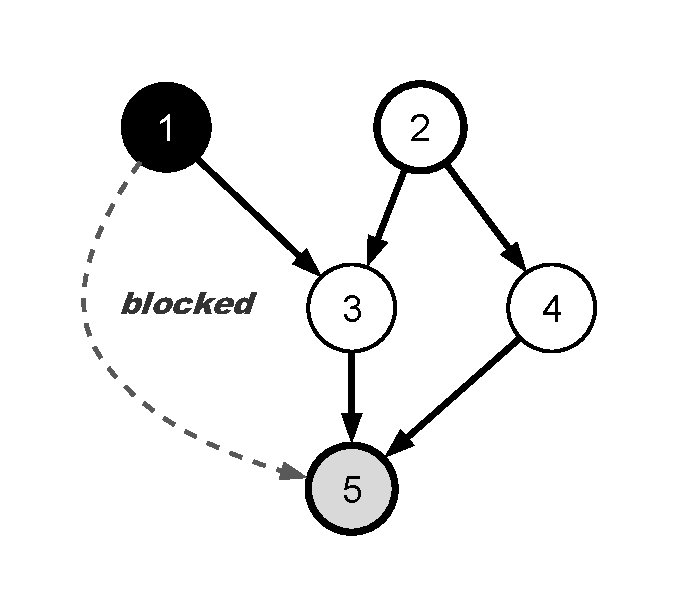
\includegraphics[width=0.42\linewidth]{fig06_edge_isolation/fig06_edge_isolation.pdf}
  \caption[Edge isolation at a nested join]{Edge isolation at join 5 in context $E=\{1\}$. Node 1 (filled) was conditioned by an enclosing diamond and is excluded from the group $G=\{3,4\}$ with fork 2. Its direct edge $(1,5)$, drawn dashed, is admitted by the first three filter clauses but blocked by the fourth. Bold edges form the nested diamond's edge list.}
  \label{fig:isolation}
\end{figure}

\subsection{Context-aware identity}
\label{sec:dd-identity}

Every diamond is identified in \texttt{unique\_diamonds} by the key
\[
\hkey(D) \;=\; \bigl(\ED,\; \{f\} \cup (E \cap R)\bigr) ,
\]
its edge list together with its \emph{relevant context}, meaning the fork it conditions on plus whatever already conditioned nodes lie in its span. The second term is what makes deduplication safe. The structural case that forces it involves a fork that is also a graph source. Such a node has no incoming edges, so the boundary cut of Section~\ref{sec:dd-edges} does nothing to it, and the same edge list arises whether that fork is being conditioned at the current level or was already fixed one level up. The two situations are different objects, one a top-level diamond and the other nested inside the diamond that did the fixing, and a key of the form $(\ED, \{f\})$ cannot tell them apart. Proposition~\ref{prop:identity} proves both that the naive key genuinely collides and that the relevant-context key separates exactly the cases that must be separated.

\subsection{The exclusion predicate \texttt{is\_det}}
\label{sec:dd-isdet}

One rule in identification consults declared node values. A node is excluded from conditioning candidacy when its reachability is already settled, which covers exactly two cases. A dead node, declared value $0$, is never active, so nothing is reached through it. A certain source, declared value $1$ with no incoming edges, is always reachable and has nothing upstream to resolve. The conjunction in the second case matters. A value-$1$ node that is not a source is still uncertain as a destination, because its reachability depends on its incoming edges, and it must remain conditionable. The simpler test of excluding every node valued $0$ or $1$ would disable every diamond in a network whose node values all happen to be $1$, a configuration that real benchmark scenarios do use. For interval-valued and p-box-valued networks the predicate is conservatively false. It is one of the three override points of Section~\ref{sec:dd-genericity}, and a user can replace it with an exclusion rule of their own.

\section{Structural Correctness}
\label{sec:dd-correctness}

All results in this section are statements about the structure of the input graph and nothing else. They divide along the line drawn in Section~\ref{sec:dd-genericity}, with termination and determinism belonging to the recursive skeleton and grouping, disjointness, and completeness to the predicates that define the diamond.

\begin{theorem}[Termination]
\label{thm:termination}
The recursion of Algorithm~\ref{alg:new-identify} terminates after at most $|V|$ nested conditioning steps along any recursive path.
\end{theorem}

\begin{proof}
Along any path of the recursion, each call either returns without recursing, which happens when every group at the join in view is a singleton, or selects a fork $f$ and recurses with $B = E \cup \{f\}$. The candidate collection of Section~\ref{sec:dd-fork} never offers a node already in $E$, so $f \notin E$ and $|V \setminus B| = |V \setminus E| - 1$ strictly. The quantity $|V \setminus E|$ is a non-negative integer that strictly decreases along the recursive path, and from its initial value $|V \setminus \varnothing| = |V|$ it admits at most $|V|$ decrements.
\end{proof}

\begin{theorem}[Grouping correctness]
\label{thm:grouping}
Fix a join $v$, context $E$, and parent set $P$. Let $H$ be the undirected graph on vertex set $P$ with an edge between $p$ and $q$ if and only if $\infl(p,E) \cap \infl(q,E) \neq \varnothing$. Then \texttt{components}$(P,E)$ returns exactly the connected components of $H$.
\end{theorem}

\begin{proof}
The procedure evaluates the intersection test for every unordered pair in $P$, which by construction is precisely the edge relation of $H$, and performs a union--find merge exactly on the pairs that pass. Union--find computes the partition of a vertex set into connected components given its edge relation. Applied to the vertices and edges of $H$, its output is the component partition of $H$.
\end{proof}

\begin{theorem}[Group disjointness]
\label{thm:disjoint}
If $G_i \neq G_j$ are distinct groups returned by \texttt{components}$(P,E)$, then
\[
\Bigl(\bigcup_{p\in G_i}\infl(p,E)\Bigr) \;\cap\; \Bigl(\bigcup_{q\in G_j}\infl(q,E)\Bigr) \;=\; \varnothing .
\]
\end{theorem}

\begin{proof}
Let $p \in G_i$ and $q \in G_j$ be arbitrary. By Theorem~\ref{thm:grouping} the two lie in different connected components of $H$, so $(p,q)$ is not an edge of $H$. Since every pair was tested directly, the test itself must have failed, giving $\infl(p,E) \cap \infl(q,E) = \varnothing$. The displayed intersection expands to the union of these pairwise intersections over all $p \in G_i$ and $q \in G_j$, and every one of them is empty.
\end{proof}

Disjointness is a statement about unconditioned influence sets, and it is what permits decomposing the groups separately. Whether separately computed values recombine correctly at the join is a different claim, which Chapter~\ref{ch:probability-toolkit} makes and proves in its own terms.

\begin{theorem}[Global completeness]
\label{thm:completeness}
Let $v$ be a join node of $G$ with parent set $P$, and suppose there exist distinct $p, q \in P$ and a node $a$ with $\lnot\texttt{is\_det}(a)$ such that either $a$ is a fork node in $\Anc(p)\cap\Anc(q)$, or $p \in \Anc(q)$ (the asymmetric case, taking $a = p$). Then the top-level pass of \texttt{new\_identify} stores a diamond for $v$ in \texttt{root\_diamonds}. Conversely, a join admitting no such pair receives no entry.
\end{theorem}

\begin{proof}
At the top level $E = \varnothing$, so in either case $a \in \infl(p,\varnothing)\cap\infl(q,\varnothing)$ and the intersection is non-empty. By Theorem~\ref{thm:grouping}, $p$ and $q$ lie in a common group $G$ with $|G|\ge 2$. In the candidate tally of Section~\ref{sec:dd-fork}, $a$ is counted once for each member it covers, so from $p$ and $q$ alone its coverage is at least $2$ and the candidate set is non-empty. A non-empty finite candidate set has a $\topi$-minimal element, so \texttt{shared\_fork} returns some fork, not necessarily $a$ itself, Algorithm~\ref{alg:new-identify} constructs a diamond for $G$, and the top-level loop records it under $v$. For the converse, if no such pair exists then every pairwise influence intersection at $v$ is empty, every group is a singleton, and the algorithm constructs nothing at $v$. That is the correct outcome, because the incoming paths of $v$ are pairwise structurally unrelated.
\end{proof}

\begin{lemma}[Edge isolation]
\label{lem:isolation}
Let $D$ be constructed for group $G$ at join $v$ under boundary $B$ as in Section~\ref{sec:dd-edges}. Then $(u,w) \in \ED$ if and only if $(u,w)\in E$, $u,w \in R$, $w \notin B$, and ($w \neq v$ or $u \in G$). Consequently every directed path within $\ED$ that terminates at $v$ has its final edge originating in $G$, and no path within $\ED$ passes through a node of $B$.
\end{lemma}

\begin{proof}
The membership characterisation restates the filter defining $\ED$. For the path properties, induct on path length. A length-one path into $v$ is a single edge $(u,v) \in \ED$, which the fourth clause forces to have $u \in G$. Any longer path has a final edge satisfying the same property, and each preceding edge $(u,w)$ has $w \notin B$ and both endpoints in $R$ by the first three clauses, so no intermediate node of the path lies in $B$ and no edge of the path enters from outside $R$.
\end{proof}

\begin{theorem}[Determinism]
\label{thm:determinism}
For a fixed input graph and iteration sets $(G, L)$, join $v$, context $E$, and admissible parent set, the diamonds returned by Algorithm~\ref{alg:new-identify} are uniquely determined, independent of set or dictionary iteration order, thread scheduling, or any other accident of execution.
\end{theorem}

\begin{proof}
By induction on recursion depth, it suffices that each step of one call is a function of its arguments alone. This holds for the partition step because, by Theorem~\ref{thm:grouping}, its output is the connected-component partition of $H$, a graph invariant that does not depend on the order in which pairs are examined or merges performed. It holds for the selection step because within each group the algorithm returns the minimum of a non-empty finite subset of $V$ under $\topi$, and a strict total order (Definition~\ref{def:topi}) admits exactly one minimum on such a set. Non-emptiness is guaranteed whenever the group has size at least two, by the tally argument of Theorem~\ref{thm:completeness}. The boundary $B = E \cup \{f\}$ and span $R$ are then determined, hence so is $\ED$, and hence so are the interior joins passed to the recursive calls, which are deterministic by the inductive hypothesis.
\end{proof}

The shape of this guarantee, a fixed total order pinning every choice point so that the output is a canonical function of the input, is also the shape of the canonicity guarantee of reduced ordered binary decision diagrams \cite{bryant1986graph}. The mechanism is not the same. BDD canonicity depends on an externally supplied variable ordering, whereas $\topi$ is derived from a property of the input graph already proved in Chapter~\ref{ch:input-module}.

\begin{proposition}[Context-aware identity: necessity and sufficiency]
\label{prop:identity}
(i) There exist graphs, a source fork $f$, and contexts $E_1 = \varnothing$ and $E_2 \ni f$ under which the construction of Section~\ref{sec:dd-edges} yields the same edge list $\ED$, while the resulting diamonds belong at different levels of the nesting hierarchy. An identity of the form $(\ED, \{f\})$ therefore conflates structurally distinct diamonds. (ii) Under $\hkey(D) = (\ED, \{f\}\cup(E\cap R))$, two constructions receive the same key only if they have the same edge list, condition on the same fork, and their contexts agree on every node of the span $R$. In that case they pose the identical sub-problem and deduplication is correct.
\end{proposition}

\begin{proof}
(i) Let $f$ be a fork that is also a graph source, and let $v$ be a join reachable from $f$ along two paths. If $f$ is free and selected at the current level, so that $E_1 = \varnothing$, the boundary cut removes the edges into $f$, of which there are none, and produces some edge list $\ED$. The diamond is top-level. If instead $f$ was conditioned by an enclosing diamond, so that $f \in E_2$, the same cut is applied for the same reason, again removes nothing, and produces the same $\ED$. This diamond is nested inside the one that fixed $f$. The pair $(\ED, \{f\})$ is identical in the two situations, but the diamonds are not interchangeable, since one must be recorded at the top level and the other inside its enclosing diamond's substructure.

(ii) Suppose $\hkey(D_1) = \hkey(D_2)$. Equality of edge lists forces equality of the spanned node sets $R$, and equality of $\{f\}\cup(E \cap R)$ then forces the two contexts to agree on every node of that shared span. Nodes outside $R$ cannot affect the diamond's interior, because by Lemma~\ref{lem:isolation} no path of $\ED$ enters from outside $R$, so a node beyond the span has no route by which to influence the pattern whether it is conditioned or not. Two constructions that agree on the edge list, the fork, and the context restricted to the span therefore define the same sub-problem, and sharing one stored entry between them loses nothing. In the collision of part (i) the enclosing construction had conditioned at least one node lying in the span, namely $f$ itself, so $E_1 \cap R \neq E_2 \cap R$ and the keys differ. The two diamonds that must be kept apart are kept apart.
\end{proof}

The key is also deliberately coarse in one direction. Constructions whose contexts differ only outside the span receive the same identity, and part (ii) is the reason this is reuse rather than a collision.

\label{sec:dd-complexity}
Taken together, these guarantees have a counting consequence. Consider a join whose $k$ parents are all mutually correlated in the naive sense, with every parent sharing some ancestry with some other. Conditioning on the shared cutset jointly means enumerating its $2^{k}$ assignments. The decomposition replaces this in two moves, both already proved. The parent set is partitioned into groups whose influence sets are disjoint (Theorems~\ref{thm:grouping} and~\ref{thm:disjoint}), so the groups decompose independently. Each group, whatever its size, is then reduced to a single conditioning fork, one fork per group rather than one per correlated pair. In the extreme case where partitioning finds $k$ separate groups, $k$ constant-size single-fork problems stand where a $2^{k}$ enumeration stood.

The identification pass itself is polynomial. Per join it computes pairwise influence intersections under union--find and builds one span, and the \texttt{unique\_diamonds} store bounds the number of distinct diamonds ever materialised. The exponential object in this problem is the downstream conditioning enumeration, and the decomposition's contribution is to make those enumerations as small and as widely reused as the network's structure allows.

\section{Representation and Reuse}
\label{sec:dd-representation}

\subsection{Diamonds as graph objects}
\label{sec:dd-selfsimilar}

Identification finds the diamonds. The module's second algorithm builds each one into a graph object of the same form as the full network. Each entry of \texttt{unique\_diamonds} is a \texttt{DiamondComputationData} carrying the complete local structural analysis of one diamond, and its fields correspond one-for-one to the unified graph object of Chapter~\ref{ch:input-module}, as Table~\ref{tab:dd-selfsimilar} shows.

\begin{table}[htbp]
\centering
\caption{Field correspondence between the unified graph object of Chapter~\ref{ch:input-module} and \texttt{DiamondComputationData}}
\label{tab:dd-selfsimilar}
\small
\renewcommand{\arraystretch}{1.15}
\begin{tabular}{|l|l|p{0.36\textwidth}|}
\hline
\textbf{Unified graph object} & \textbf{Diamond entry} & \textbf{Role} \\
\hline
\texttt{outgoing\_index} & \texttt{sub\_outgoing\_index} & Forward adjacency \\
\texttt{incoming\_index} & \texttt{sub\_incoming\_index} & Reverse adjacency \\
\texttt{source\_nodes} & \texttt{sub\_sources} & Local sources of the span \\
\texttt{fork\_nodes} & \texttt{sub\_fork\_nodes} & Local forks \\
\texttt{join\_nodes} & \texttt{sub\_join\_nodes} & Local joins \\
\texttt{ancestors} & \texttt{sub\_ancestors} & Closure restricted to the span \\
\texttt{descendants} & \texttt{sub\_descendants} & Closure restricted to the span \\
\texttt{iteration\_sets} & \texttt{sub\_iteration\_sets} & Layered order restricted to the span \\
\texttt{node\_priors} & \texttt{sub\_node\_priors} & Value map restricted to the span \\
--- & \texttt{sub\_diamond\_structures} & Nested diamonds interior to this one \\
\hline
\end{tabular}
\end{table}

Because a diamond satisfies the same object contract as the network it came from, anything the framework can do with the full network it can do with a diamond, including decomposing it further, which is what the recursion does. The analysis recorded in Table~\ref{tab:dd-selfsimilar} is paid for once at identification time and reused on every later consultation.

\label{sec:dd-supernode}
The reductive use of a diamond noted in Section~\ref{sec:dd-family} rests on the same contract. A solved diamond can stand in the parent graph as a single equivalent node precisely because it satisfies that contract. Identification establishes only the compatibility, since performing the substitution needs a solved value, which structure alone cannot supply.

\subsection{Deduplication by hash-consing}
\label{sec:dd-hashconsing}

Before constructing a new entry, the algorithm looks the diamond's key up in \texttt{unique\_diamonds}. A structurally identical diamond already resolved anywhere else in the recursion, under another maximal diamond or at another nesting level, is referenced rather than rebuilt. This is hash-consing in the standard sense \cite{ershov1958programming,filliatre2006hashconsing}, a table keyed by structural identity so that equal structures are stored once and identity comparison becomes a key comparison. The same technique appears as the unique table of a BDD package. Without the store the recursion is a tree and every call site is distinct. With it, structurally identical call sites collapse into shared entries and the representation becomes a DAG. The collapse loses nothing, because by Proposition~\ref{prop:identity}(ii) two call sites receive the same key only when they pose the identical sub-problem.

\section{Worked Examples}
\label{sec:dd-examples}

\subsection{The atomic diamond}
\label{sec:dd-atomic}

Figure~\ref{fig:atomic} shows the minimal pattern, a source $s$ feeding a fork $f$, two internally disjoint paths $\alpha$ and $\beta$, and a join $j$ where they meet. At $j$ both parents' influence sets contain $f$, so the parents form one group. Fork $f$ is the only covering candidate, it is selected, and the diamond spans the whole figure with $C = \{f\}$.

\begin{figure}[htbp]
  \centering
  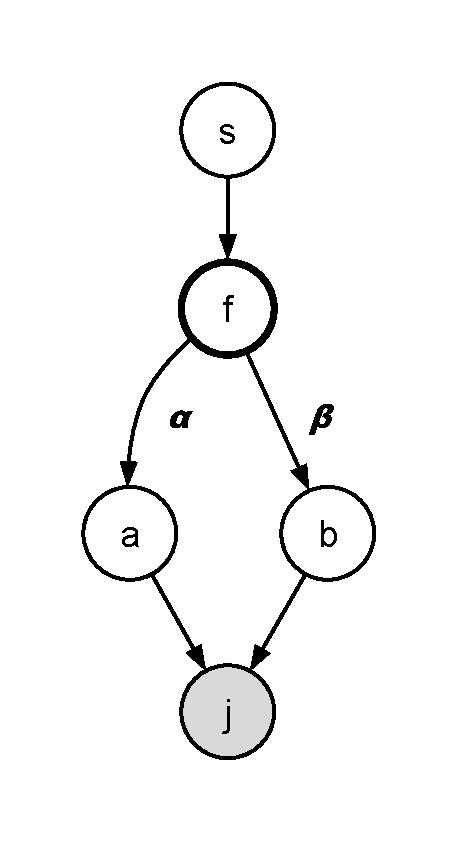
\includegraphics[width=0.3\linewidth]{fig01_atomic_diamond/fig01_atomic_diamond.pdf}
  \caption{The atomic diamond.}
  \label{fig:atomic}
\end{figure}

\subsection{A nested decomposition}
\label{sec:dd-nested-example}

The eight-node network of Figure~\ref{fig:nested-full} has forks 1 and 3 and joins 6 and 8. An outer reconvergence runs through fork 1 and meets at join 8, and on one of its branches an inner reconvergence runs through fork 3 and meets at join 6. The decomposition below is not hand-derived. It is the output of the implementation on this edge list, machine-checked, and the example of Figure~\ref{fig:isolation} was verified in the same run.

\begin{figure}[htbp]
  \centering
  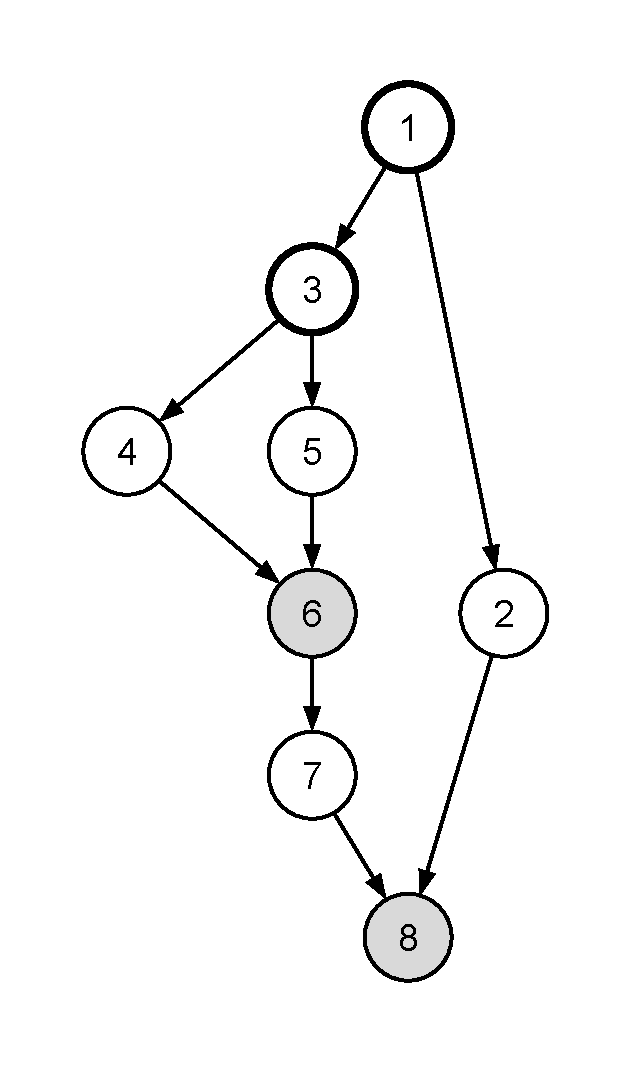
\includegraphics[width=0.34\linewidth]{fig02_nested_full/fig02_nested_full.pdf}
  \caption{Frame 1. The network, with forks outlined in bold and joins shaded.}
  \label{fig:nested-full}
\end{figure}

\textbf{Join 8, top level.} The parents are $\{2,7\}$, with $\infl(2,\varnothing) = \{1,2\}$ and $\infl(7,\varnothing) = \{1,3,4,5,6,7\}$. The sets intersect in $\{1\}$, so the parents form one group. Fork 1 is the only candidate covering both and is selected, and the maximal diamond $D_1$ spans all nine edges with $C = \{1\}$ (Figure~\ref{fig:nested-outer}).

\begin{figure}[htbp]
  \centering
  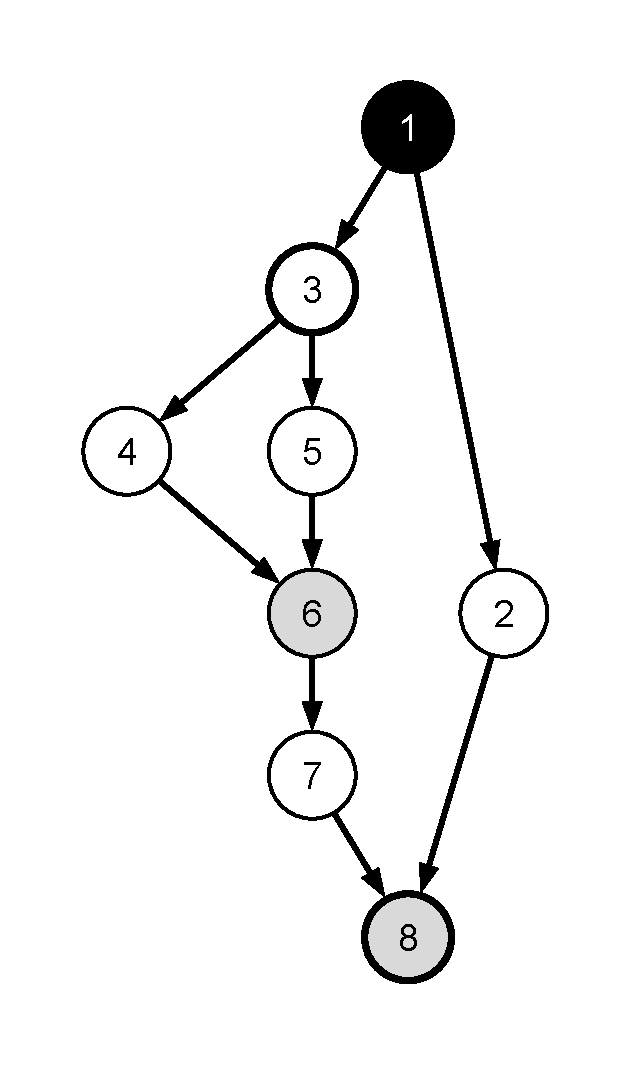
\includegraphics[width=0.36\linewidth]{fig03_nested_outer/fig03_nested_outer.pdf}
  \caption{Frame 2. The maximal diamond at join 8, with fork 1 conditioned (filled) and the span covering the whole network.}
  \label{fig:nested-outer}
\end{figure}

\textbf{Join 6, inside $D_1$.} Under the boundary $B = \{1\}$, interior join 6 has parents $\{4,5\}$ with $\infl(4,\{1\}) = \{3,4\}$ and $\infl(5,\{1\}) = \{3,5\}$. The parents are still correlated through fork 3, so conditioning on 1 did not resolve the inner reconvergence, and this is the case the recursion exists for. The recursive call selects fork 3 and produces the inner diamond $D_3$ with $C = \{3\}$ and $\ED = \{(3,4),(3,5),(4,6),(5,6)\}$. The edge $(1,3)$ is cut by the boundary clause because its head is conditioned at this level (Figure~\ref{fig:nested-inner}).

\begin{figure}[htbp]
  \centering
  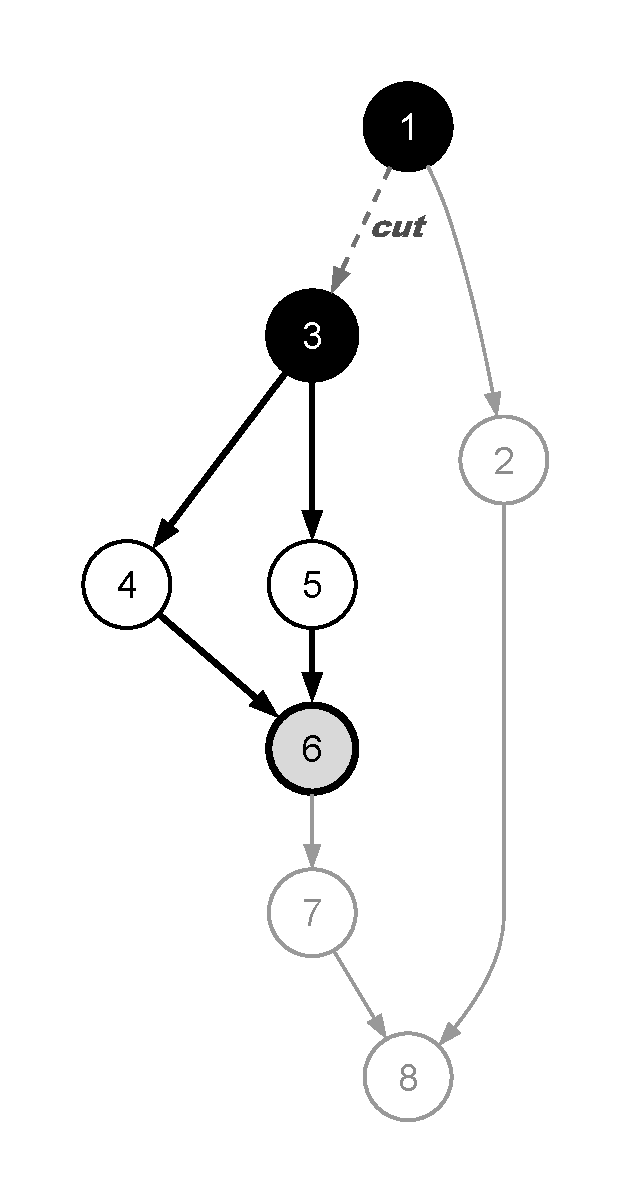
\includegraphics[width=0.36\linewidth]{fig04_nested_inner/fig04_nested_inner.pdf}
  \caption{Frame 3. The recursive call at join 6 in context $E=\{1\}$, with fork 3 selected, the inner diamond in bold, and edge $(1,3)$ cut.}
  \label{fig:nested-inner}
\end{figure}

\textbf{Join 6, top level.} Join 6 is also a join of the network itself, so the top-level pass visits it in its own right, and here the candidate set is larger. With $E = \varnothing$, forks 1 and 3 both cover parents 4 and 5, and the minimum-$\topi$ rule of Section~\ref{sec:dd-fork} selects fork 1, the covering node closest to the source, rather than fork 3, which a reader tracing by eye might expect. The result is a second maximal diamond $D_2$ spanning $\{(1,3),(3,4),(3,5),(4,6),(5,6)\}$ with $C = \{1\}$, and its interior recursion, now in context $\{1\}$, again produces exactly $D_3$.

\textbf{The emitted hierarchy.} In total the module returns two maximal diamonds and three unique diamonds (Figure~\ref{fig:hierarchy}). $D_1$ sits at join 8 and $D_2$ at join 6, each with $C=\{1\}$. The inner $D_3$ at join 6 with $C=\{3\}$ is stored once and referenced from the substructure tables of both $D_1$ and $D_2$ under the same key. Two different enclosing recursions posed the same sub-problem, with the same edge list, the same fork, and contexts agreeing on the span, and Proposition~\ref{prop:identity}(ii) is the reason the single shared entry is correct.

\begin{figure}[htbp]
  \centering
  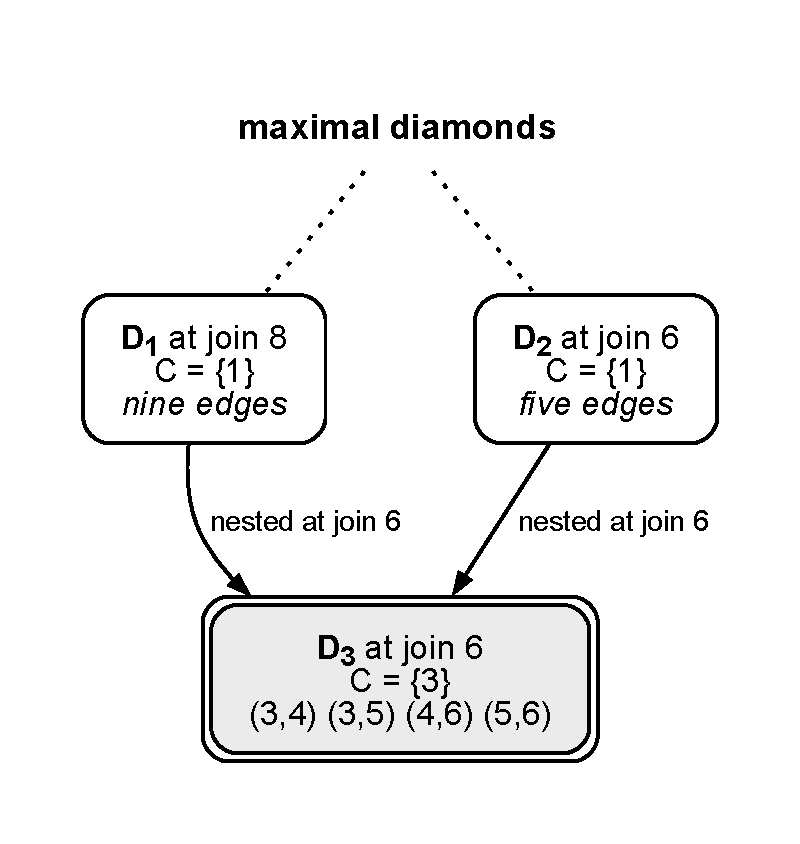
\includegraphics[width=0.6\linewidth]{fig05_hierarchy/fig05_hierarchy.pdf}
  \caption{Frame 4. The emitted hierarchy of two maximal diamonds, with the inner diamond $D_3$ stored once and referenced by both.}
  \label{fig:hierarchy}
\end{figure}

The trace also confirms the edge-isolation case of Section~\ref{sec:dd-edges} end to end. In the network of Figure~\ref{fig:isolation}, the nested diamond at join 5 under $E=\{1\}$ is emitted with $C = \{2\}\cup(\{1\}\cap R) = \{1,2\}$, which is the context-aware identity visible in the output. Node 1 is recorded as a non-diamond parent, and the edge $(1,5)$ appears in no diamond edge list.

\section{Summary}
\label{sec:dd-summary}

The module turns the graph object of Chapter~\ref{ch:input-module} into two structures. \texttt{root\_diamonds} records the network's maximal diamonds, and \texttt{unique\_diamonds} stores every diamond found at any level exactly once, each entry a graph object of the same form as the network it came from. The decomposition terminates within $|V|$ nested steps and is canonical for a given input (Theorems~\ref{thm:termination} and~\ref{thm:determinism}). It groups a join's parents exactly by unconditioned shared ancestry and produces a diamond wherever reconvergence exists and only there (Theorems~\ref{thm:grouping}--\ref{thm:completeness}). Nothing outside a diamond's span enters its edge list (Lemma~\ref{lem:isolation}), and stored structure is shared exactly when sharing is correct (Proposition~\ref{prop:identity}). At a join of $k$ correlated parents the result is $k$ single-fork conditioning problems in place of one $2^{k}$ enumeration.

Two questions are left open deliberately. One is how the values of independently decomposed groups recombine at a join. The other is the substitution of a solved diamond back into its parent graph as a single equivalent component. Both need values as well as structure, and the Probability Propagation Toolkit takes them up.

\ifdefined\maindoc
% do nothing
\else
\printbibliography
\end{document}
\fi
